% ============================================================================
\section{Inference memory and attention variants}
% ============================================================================

% --- MHA MQA GQA + table ---
% \begin{frame}{MHA, MQA, and GQA: shrinking the KV cache}
%   \begin{itemize}
%     \item \textbf{MHA:} $h$ query heads each with their own $K,V$ projections: KV cache stores $h$ copies---memory-heavy for long contexts.
%     \item \textbf{MQA:} single shared $K,V$ across heads (Shazeer et al.); cuts KV memory; may need re-tuning.
%     \item \textbf{GQA:} group heads so each \textbf{group} shares KV (Ainslie et al.): quality--bandwidth trade-off; widely deployed (LLaMA~2/3-class stacks).
%   \end{itemize}
%   \centering
%   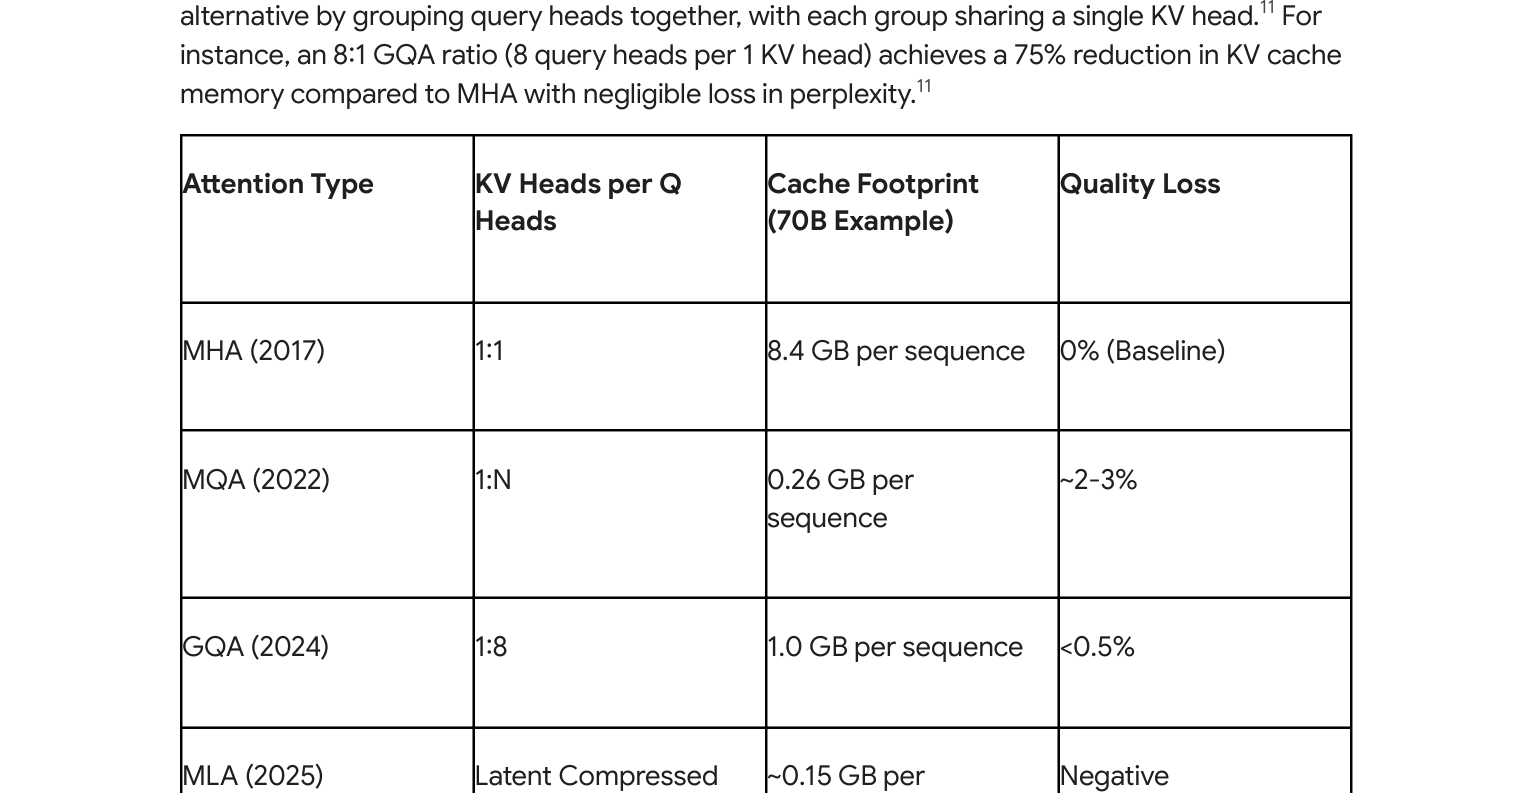
\includegraphics[width=\textwidth,height=0.38\textheight,keepaspectratio]{assets/New-Lecture-Transformers/report_crop_kv_attention_table.png}
% \end{frame}

\begin{frame}{Key-Value Caching}
  \begin{columns}[T,onlytextwidth]
    \column{0.48\textwidth}
    \begin{itemize}\itemsep0.32em
      \item[\textcolor{red}{$\blacktriangleright$}] In \textbf{decode}, the model emits \textbf{one token per step}, but that token still depends on the \textbf{key and value} tensors for \textbf{all} earlier positions.
      \item[\textcolor{red}{$\blacktriangleright$}] Those positions include the \textbf{prompt} (K/V from \textbf{prefill}) plus any \textbf{new} K/V computed up to the current step.
      \item[\textcolor{red}{$\blacktriangleright$}] \textbf{KV caching} keeps these tensors in GPU memory so they are \textbf{not recomputed} at every step; each iteration \textbf{appends} the newly computed K/V to the cache for the next step.
      \item[\textcolor{red}{$\blacktriangleright$}] In many stacks there is \textbf{one KV cache per transformer layer}.
    \end{itemize}
    \vspace{0.2em}
    {\scriptsize Verma \& Vaidya, ``Mastering LLM Techniques: Inference Optimization,'' NVIDIA Technical Blog (2023). \href{https://developer.nvidia.com/blog/mastering-llm-techniques-inference-optimization/}{Article} --- Key-value caching (Figure~1).}

    \column{0.5\textwidth}
    \centering
    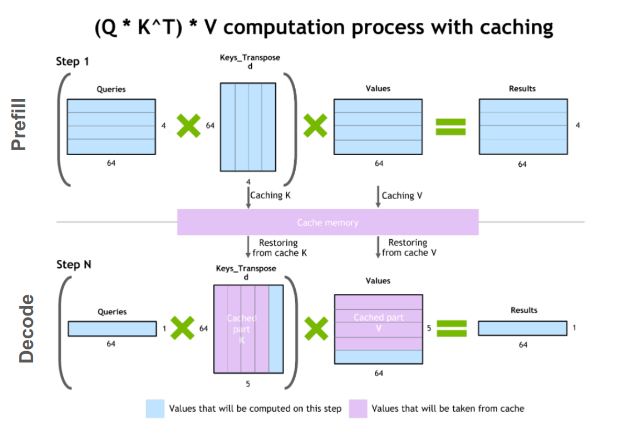
\includegraphics[width=0.8\linewidth,height=0.78\textheight,keepaspectratio]{assets/New-Lecture-Inference_Optimisation/nvidia_blog_kv_caching_figure1.png}\\[-0.2em]
    {\scriptsize Figure~1: illustration of the key-value caching mechanism.}
  \end{columns}
\end{frame}

\begin{frame}{KV Cache Memory}
  \begin{columns}[T,onlytextwidth]
    \column{0.52\textwidth}
    \begin{itemize}\itemsep0.28em
      \item[\textcolor{red}{$\blacktriangleright$}] Major GPU memory uses for serving: \textbf{model weights} and the \textbf{KV cache} (self-attention tensors cached to skip redundant work).
      \item[\textcolor{red}{$\blacktriangleright$}] Under batching, each request still needs a \textbf{separate} KV-cache allocation---often the limiting factor before weights alone.
      \item[\textcolor{red}{$\blacktriangleright$}] Cost scales \textbf{linearly} with batch and length---caps throughput and long-context use; motivates MQA/GQA, paging (PagedAttention), KV quantisation, etc.
      \end{itemize}
    \column{0.47\textwidth}
    \centering
    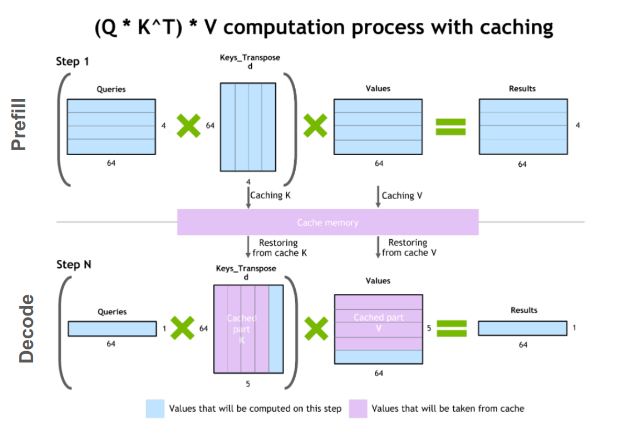
\includegraphics[width=0.8\linewidth,height=0.78\textheight,keepaspectratio]{assets/New-Lecture-Inference_Optimisation/nvidia_blog_kv_caching_figure1.png}\\[-0.2em]
    {\scriptsize Figure~1: illustration of the key-value caching mechanism (from previous frame).}
  \end{columns}
\end{frame}

\begin{frame}{MHA, MQA, GQA: shrinking the KV cache}
  \centering
  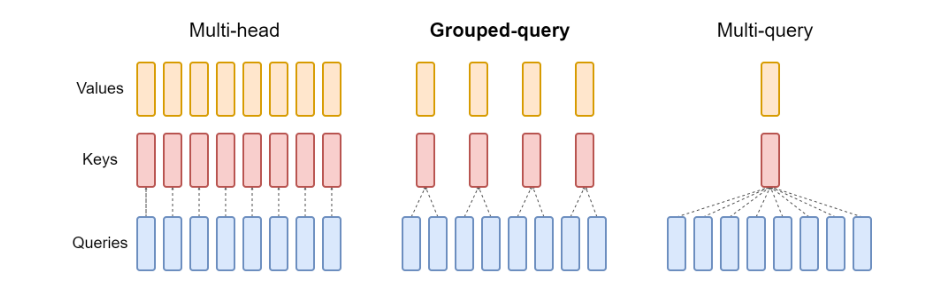
\includegraphics[width=\textwidth,height=0.78\textheight,keepaspectratio]{assets/New-Lecture-Transformers/gqa_paper_page_2.png}
  {\scriptsize
    \begin{itemize}
      \item \textbf{Multi-head attention (MHA)}: $H$ separate query, key, and value heads.
      \item \textbf{Multi-query attention (MQA)}: single shared key and value heads for all query heads.
      \item \textbf{Grouped-query attention (GQA)}: shares key and value heads for each \textit{group} of query heads.
      \item GQA conceptually interpolates between multi-head and multi-query attention.
    \end{itemize}
  }
  {\scriptsize \textit{Reference:} 
    Ainslie et al., ``GQA: Training Generalized Multi-Query Transformer Models from Multi-Head Checkpoints,'' 
    \href{https://arxiv.org/abs/2305.13245}{arXiv:2305.13245}.
  }
\end{frame}

% \begin{frame}{Multi-Head Latent Attention (MLA)}
%   \begin{itemize}
%     \item \textbf{Idea:} compress $K,V$ into a \textbf{low-rank latent} before cache storage; project back during attention. Targets the same bottleneck as MQA/GQA---KV memory---with a learned compression map.
%     \item Reported serving stacks claim \textbf{smaller cache footprints} than GQA at similar or better quality on some large-model regimes (see DeepSeek-V3 technical report and follow-on discussions).
%     \item Pedagogically: MLA is ``KV compression + multi-head expressivity,'' not only ``share heads.''
%   \end{itemize}
% \end{frame}

% \begin{frame}{KV cache and PagedAttention}
%   \begin{itemize}
%     \item Autoregressive decoding caches past \textbf{key/value} tensors so each new token only computes one new column of attention against history.
%     \item Memory $\propto$ \textbf{layers} $\times$ \textbf{batch} $\times$ \textbf{context length} $\times$ \textbf{KV head dim}; \textbf{MQA/GQA/MLA} directly change the last factor.
%     \item \textbf{PagedAttention} (vLLM): store KV in non-contiguous blocks like OS virtual memory---reduces internal fragmentation from reserving max-length buffers; large reported cuts in wasted GPU memory for variable-length serving.
%     \item Systems stack: prefix caching, speculative decoding, expert parallelism for MoE---as important as raw model FLOPs.
%   \end{itemize}
% \end{frame}

% \begin{frame}{Transformer Variants}
%   \begin{itemize}
%     \item[$\blacktriangleright$] \textbf{Encoder-only:} BERT, RoBERTa
%     \item[$\blacktriangleright$] \textbf{Decoder-only:} GPT, LLaMA, Falcon
%     \item[$\blacktriangleright$] \textbf{Encoder-Decoder:} T5, BART, mT5
%   \end{itemize}
%   \vspace{1em}
%   \textbf{Modifications:}
%   \begin{itemize}
%     \item[$\blacktriangleright$] \textbf{Long-range:} Longformer, BigBird
%     \item[$\blacktriangleright$] \textbf{Efficient:} Linformer, Performer
%     \item[$\blacktriangleright$] \textbf{Sparse:} Sparse Transformer, Reformer
%   \end{itemize}
% \end{frame}

\begin{frame}{The LLM Era -- Paradigm Shift in Machine Learning}
  \centering
  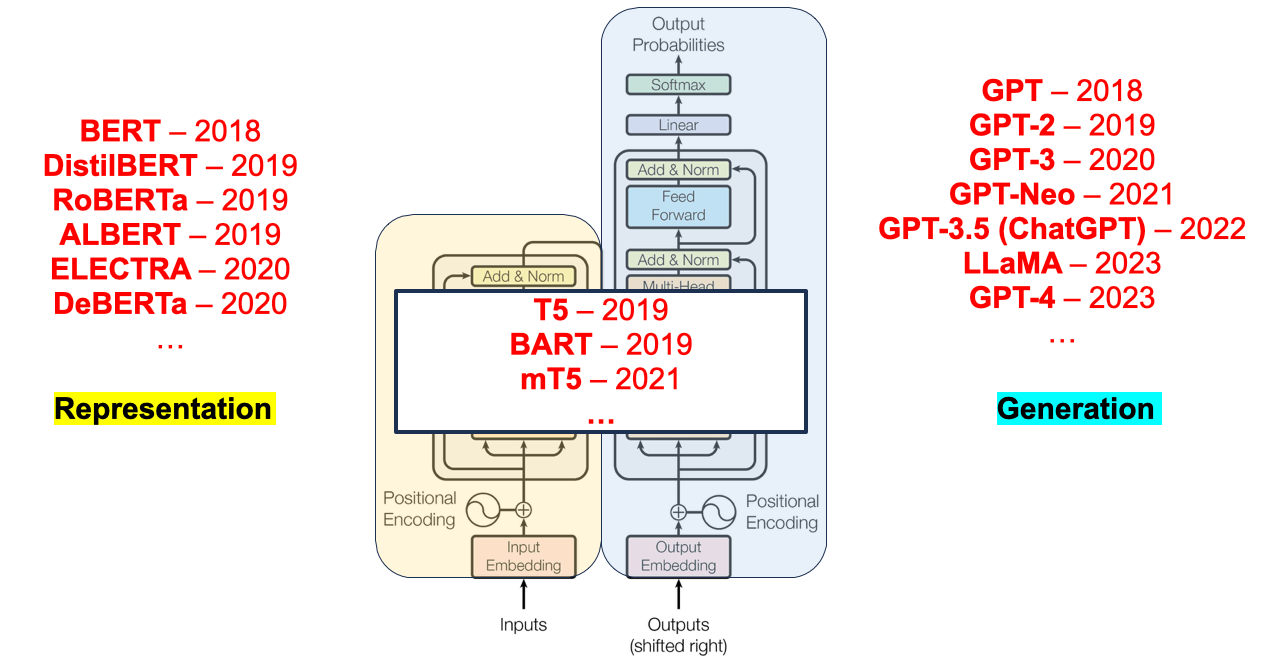
\includegraphics[width=0.8\paperwidth,height=0.8\paperheight,keepaspectratio]{assets/Lecture-6_Introduction_to_Transformers/pdf_page_095.png}
\end{frame}


\begin{frame}{Decoder-only LLMs (post-2017 trend)}
  \begin{itemize}
    \item GPT-style \textbf{causal (masked) self-attention}: each token attends only to the past.
    \item Single stack replaces separate encoder/decoder for many language (and vision--language) workloads.
    \item Encoder--decoder Transformers remain standard in \textbf{seq2seq} (MT, Whisper ASR, some VL captioning) where cross-attention helps.
  \end{itemize}
\end{frame}
